
\chapter{Bibliographic revision}

\section{Fair Machine Learning}

The field of Machine Learning (ML) has experienced significant growth and is increasingly applied in various societal domains such as healthcare, finance, and criminal justice. This growth raises important ethical and operational concerns, particularly regarding the principles of Fairness, Accountability, and Transparency (FAT) \citep{}. As ML algorithms increasingly influence a wide array of societal domains, including criminal justice, healthcare, finance, and employment, the imperative to ensure these systems are designed and implemented responsibly has become paramount. This section aims to delineate the significance, scope, and prevailing challenges associated with integrating FAT principles into ML, providing a foundation for the subsequent discussion.

Fairness in ML concerns the equitable and just treatment of all individuals, particularly those from historically marginalized or disadvantaged groups\citep{}. It seeks to ensure that ML algorithms do not perpetuate existing biases or create new forms of discrimination. However, the multifaceted nature of fairness, encompassing various definitions and metrics, poses substantial challenges in operationalizing it within algorithmic frameworks. Further in this section we will explore these complexities, examining different conceptions of fairness and the inherent trade-offs they entail.

Accountability in ML pertains to the obligation of designers, developers, and deployers of ML systems to be answerable for the outcomes of these systems\citep{}. It involves establishing mechanisms that allow for the tracing of decisions back to the entities responsible for the deployment of the ML algorithms. Accountability also encompasses the adherence to ethical standards, legal requirements, and societal norms. This discussion frequently involves mechanisms and practices that can enhance accountability in ML, like auditing, documentation, and regulatory compliance.

Transparency, the third pillar, refers to the clarity and openness with which ML systems operate\citep{}. It involves the ability of stakeholders, including end-users, regulators, and the broader public, to understand how ML systems make decisions. Transparency is crucial for building trust, facilitating informed consent, and enabling the scrutiny necessary to identify and rectify biases. However, achieving transparency, particularly with complex models, presents its own set of technical and ethical challenges. This research topic includes isses as the trade-off between explainability and model performance, and discussing emerging approaches to enhance interpretability without sacrificing effectiveness.

The triad of Fairness, Accountability, and Transparency (FAT) alongwith data privacy forms the cornerstone of Trustworty Artificial Intelligence (TwAI). These principles are pivotal in ensuring that AI systems are developed and deployed in a manner that respects human rights, promotes social well-being, and maintains public trust. While accountability ensures that entities behind AI systems can be held responsible for their outcomes, transparency allows stakeholders to understayfoster environments where AI systems can be scrutinized, understood, and corrected, thereby aligning their functionality with societal norms and values. 

In this context of Trustworty AI the European Union's High-Level Expert Group on Artificial Intelligence has outlined seven key principles that aim to ensure that AI systems are designed and used in a way that is ethically sound and trustworthy~\citep{TwAI_Europe}. These principles are crucial for building AI systems that are beneficial and do not cause unintended harm. The seven principles are as follows:

\begin{description}
    \item[Human agency and oversight] AI systems should empower human beings, allowing them to make informed decisions and fostering their fundamental rights. At the same time, proper oversight mechanisms need to be ensured, which can be achieved through human-in-the-loop, human-on-the-loop, and human-in-command approaches
    \item[Technical Robustness and safety] AI systems need to be resilient and secure. They need to be safe, ensuring a fall back plan in case something goes wrong, as well as being accurate, reliable and reproducible. That is the only way to ensure that also unintentional harm can be minimized and prevented.
    \item[Privacy and data governance] besides ensuring full respect for privacy and data protection, adequate data governance mechanisms must also be ensured, taking into account the quality and integrity of the data, and ensuring legitimised access to data.
    \item[Transparency] the data, system and AI business models should be transparent. Traceability mechanisms can help achieving this. Moreover, AI systems and their decisions should be explained in a manner adapted to the stakeholder concerned. Humans need to be aware that they are interacting with an AI system, and must be informed of the system’s capabilities and limitations.
    \item[Diversity, non-discrimination and fairness] Unfair bias must be avoided, as it could could have multiple negative implications, from the marginalization of vulnerable groups, to the exacerbation of prejudice and discrimination. Fostering diversity, AI systems should be accessible to all, regardless of any disability, and involve relevant stakeholders throughout their entire life circle.
    \item[Societal and environmental well-being] AI systems should benefit all human beings, including future generations. It must hence be ensured that they are sustainable and environmentally friendly. Moreover, they should take into account the environment, including other living beings, and their social and societal impact should be carefully considered. 
    \item[Accountability] Mechanisms should be put in place to ensure responsibility and accountability for AI systems and their outcomes. Auditability, which enables the assessment of algorithms, data and design processes plays a key role therein, especially in critical applications. Moreover, adequate an accessible redress should be ensured.
\end{description}


Although there are many aspects to consider to an ethical automated decision system with social impacts, the present text will concentrate predominantly on the aspect of fairness Fairness is not only crucial for the development of just and equitable technological solutions but also imperative for maintaining the legitimacy and acceptability of AI systems in diverse societal contexts. In delving into the multifaceted dimensions of fairness, this text aims to unpack the theoretical underpinnings, practical challenges, and potential pathways to achieving fairer AI systems, thereby contributing to the broader discourse on ethical AI.

\subsection{Sources and types of algorithmic unfairness}


The comprehensive survey conducted by \citet{Mehrabi2019} elucidates the multitude of biases that can pervade artificial intelligence applications, potentially leading to unfair outcomes. This analysis categorizes the various sources of bias, illustrating the multifaceted ways in which such biases can infiltrate different stages of machine learning processes, ranging from the initial data collection phase to the final algorithmic processing. The following exposition provides a short delineation of these sources of bias. To a rich discussion on this topic - including references, examples and real cases where each source of bias can emerge - we recommend the reading of the original work. The discussion here is with the purpose of proper describing the complexity and multifaceted nature of unfairness in machine learning models.


\begin{description}
    \item[Historical Bias] This is the existing societal bias that reflects past and present inequalities and prejudices. Historical bias is present in the data even before any machine learning model has interacted with it, due to inherent social and cultural inequalities;
    
    \item[Representation Bias] Occurs when the data sample does not accurately represent the entire population or certain subgroups within it. This can lead to machine learning models that perform well on majority groups but poorly on underrepresented groups;

    \item[Measurement Bias] Arises when the data collected does not accurately measure the real-world constructs it purports to measure. This type of bias can occur due to flawed data collection instruments or processes that systematically misrepresent certain groups;
    
    \item[Evaluation Bias] This type of bias occurs during the performance evaluation of machine learning models, where the evaluation criteria or methods may favor one group over others, leading to biased assessments of model performance;

    \item[Aggregation Bias] Happens when incorrect assumptions are made about the homogeneity of groups within the data. Aggregation bias can lead to misleading conclusions if the differences within and between groups or subgroups are not properly accounted for;
    
    \item[Population Bias] Similar to representation bias, population bias occurs when statistics, demographics, representatives, and user characteristics are different in the user population represented in the dataset, leading to models that are not generalizable across different demographic groups;

    \item[Simpson’s Paradox] This is a statistical phenomenon where a trend appears in several different groups of data but disappears or reverses when these groups are combined;

    \item[Longitudinal Data Fallacy] Occurs when cross-sectional data is treated as longitudinal, leading to incorrect conclusions about data trends over time;

    \item[Sampling Bias] Introduced by non-random sampling procedures, where certain members of the intended population are less likely to be included in the sample than others, leading to skewed data that does not accurately represent the entire population;
    
    \item[Behavioral Bias] Arises from variations in user behavior that differ across different platforms or contexts, affecting the data's representation of real-world phenomena;

    \item[Content Production Bias] Results from differences in how content is generated by different groups, with structural, lexical, semantic, and syntactic differences, influencing the data available for machine learning models; 

    \item[Linking Bias] Occurs in networked data, where the connections between nodes can misrepresent the true attributes or behavior of the nodes;

    \item[Temporal Bias] Reflects changes in data characteristics over time, due changes in representation or behaviors, which may not be accounted for in static machine learning models;
    
    \item[Popularity Bias] Occurs when popular items are more likely to be recommended or rated highly, not necessarily because of their quality but simply because of their initial, higher visibility and these popularity metrics are subject of mapinupation;

    \item[Algorithmic Bias] Introduced by the algorithms themselves, when they add bias that was not present in the input data:

    \item[User Interaction Bias] Results from the way system design influences user behavior in biased ways. This source of bias can be influenced by other types or subtypes, such as Presentation and Ranking Biasese:
    \begin{description}
        \item[Presentation Bias] This bias occurs when the way information is presented influences the outcomes. In machine learning, this can manifest through the design of user interfaces or the manner in which data is displayed, affecting user decisions and interactions;

        \item[Ranking Bias] Arises when algorithms prioritize certain data points over others in ranked lists or search results, which can distort visibility and perpetuate certain preferences or discriminations;
    \end{description}
    
    \item[Social Bias] Social biases are the preconceived notions and stereotypes held by societies, where individual actions or contents are socially influenced. These biases often find their way into data through collective social behaviors and decisions, influencing the training data used for machine learning models;

    \item[Emergent Bias] Emerges during the operation of a system, particularly as a result of changes in population, cultural values, or societal knowledge in the data over time. This type of bias is dynamic and can occur even if the initial model was unbiased, due to changes in the underlying data or context;

    \item[Self-Selection Bias] Occurs when the individuals selected for a study or dataset have self-selected in some way, producing a sample that is not representative of the general population. This can skew results and make the data less generalizable;

    \item[Omitted Variable Bias] Happens when a model overlooks certain relevant variables that are correlated with both the independent and dependent variables. Omitting these variables can lead to incorrect inferences about correlations and effects;

    \item[Cause-Effect Bias] This bias is a misunderstanding in the determination of causation; it can occur when correlations are mistaken for causal relationships without proper justification through causal inference techniques;

    \item[Observer Bias] Introduced by the expectations or preconceptions of those collecting or processing data, which can influence the outcomes subconsciously.;
    
    \item[Funding Bias] Refers to the influence that the source of funding can have on the conduct of research or development of algorithms. This type of bias can lead to results that favor the interests of the funding source, consciously or unconsciously.
\end{description}

These biases can pervade various stages of machine learning, from data collection to model evaluation and deployment, highlighting the importance of understanding and mitigating bias to achieve fairness in AI systems. Furthermore, the presence of biases can lead to feedback loops that exacerbate these inequalities over time. When biased data influence the decisions made by an AI system, these decisions can then be used to generate more data, which, if used to retrain the model, may reinforce and even amplify the existing biases. This cycle can create a self-perpetuating loop, making initial biases more entrenched and difficult to correct. Addressing feedback loops is critical, as they can progressively deteriorate the fairness of the system, leading to increasingly skewed outcomes that are harder to rectify. Effective strategies to break these loops include rigorous monitoring of model decisions, regular updates to training datasets to ensure diversity and representativeness, and the implementation of mechanisms that can detect and correct for emerging biases

Having outlined the various sources of unfairness in machine learning, \citet{Mehrabi2019} also delves into the different types of discrimination that arise from these biases. Understanding these types of discrimination is crucial as they elucidate how biases, whether direct, indirect, systemic, statistical, explainable, or unexplainable, can culminate in unfair outcomes. Each type of discrimination demonstrates a distinct pathway through which biases embedded in data or algorithms manifest in practices and decisions, thus potentially perpetuating unfairness in AI systems. This comprehensive analysis helps in identifying targeted strategies to mitigate these discriminatory effects and underscores the importance of developing automated decision systems that are both just and equitable.


\begin{description}
    \item[Direct Discrimination] occurs when outcomes are directly affected by sensitive attributes such as race, gender, or age. This type of discrimination happens explicitly and is frequently legally prohibited;
    
    \item[Indirect Discrimination] manifests when proxy attributes indirectly linked to sensitive attributes influence outcomes. For example, using zip codes in decision-making processes might inadvertently reflect racial biases because residential areas often correlate with racial demographics. This phenomena is also refered as redlining effect~\citep{Pedreschi2008};
    
    \item[Systemic Discrimination] involves policies or practices entrenched within an organization that perpetuate disadvantage for certain groups. This can stem from cultural biases embedded in the decision-making processes, often reflecting the preferences or biases of dominant groups;
    
    \item[Statistical Discrimination] refers to the use of general statistics on a group to make inferences about individuals from that group. This type of discrimination might arise when decision-makers use visible characteristics as proxies for other traits, leading to biased assessments;
    
    \item[Explainable Discrimination] is considered legally permissible if the differences in treatment or outcomes can be justified through legitimate and relevant attributes. For instance, differences in pay might be justified by the number of hours worked if this factor significantly influences earnings;
    
    \item[Unexplainable Discrimination] occurs when there is no justifiable reason for the disparate treatment or outcomes, making it illegal and ethically unacceptable. This type of discrimination requires interventions to ensure fairness and equality in decision-making processes.
\end{description}


\subsection{Fairness definitions and metrics}

This section aims to present some widely used definitions and metrics of fairness, as described by \cite{Verma2018} and summarized by \cite{Mehrabi2019} and \cite{caton2023}, providing a comprehensive overview for understanding and navigating the multifaceted dimensions of fairness in ML systems. Initially, the discourse will delve into general considerations and intuitive aspects of fairness, setting the stage for a deeper understanding. This preliminary discussion is crucial as it lays the groundwork for grasping the nuanced nature of fairness notions within the context of ML. Following this, we will transition into formal definitions, where we will dissect and explain those metrics and concepts.

Even before this discussion, it's crucial to understand that no single fairness definition universally applies to all scenarios. The choice of a particular fairness definition and metric should be informed by ethical considerations grounded in the social context in which the model would be deployed~\citep{AlerTubella2022}. Selecting a fairness definition is not a purely technical matter, as it inevitably entails ethical and social considerations that should not be neglected~\citep{Alves2023}. Building fair machine learning models requires an interdisciplinary approach that engages all stakeholders, including specially those who are typically marginalized or underrepresented~\citep{Weinberg2022}.

A prevalent taxonomy within fairness literature differentiates fairness notions into group metrics and individual metrics. Group Fairness Metrics hinge on the principle that statistical measures — such as error rates, precision, and recall — ought to be equitably distributed across groups demarcated by sensitive attributes like race, gender, or age. The core premise of these metrics is that fairness is actualized when an algorithm exhibits consistent performance across diverse demographic segments.

Demographic Parity, for example, mandates uniformity in the rate of positive algorithmic outcomes across different groups, a standard that remains agnostic to the underlying base rates within each population segment. On the other hand, Equal Opportunity and Equalized Odds introduce a nuance to this conversation by tethering fairness to the true condition of outcomes. This refinement underscores a crucial differentiation within fairness metrics: some are predicated solely on predicted values (such as Demographic Parity), while others derive from the comprehensive landscape of the confusion matrix (Table~\ref{tab:confusion_matrix_definition}), incorporating true conditions (as seen in Equal Opportunity and Equalized Odds).

Individual Fairness Metrics, in contrast, introduce a more granular perspective to fairness, advocating that similar individuals should be treated similarly by the ML system. This approach diverges from group-level considerations, focusing instead on ensuring that the algorithm’s treatment is consistent for individuals who are alike in relevant aspects, barring their membership in different demographic categories. Individual fairness seeks to ensure a personalized sense of justice, where the algorithmic outcomes are solely reflective of pertinent attributes rather than biased by irrelevant factors associated with sensitive attributes. This concept champions the notion that fairness extends beyond group identities to recognize and respect the uniqueness of individual experiences and qualifications.

To establish the foundation for discussing fairness definitions and metrics, we commence with an examination of the confusion matrix, which is an essential instrument in machine learning to assessing the performance of classification algorithms. It constitutes a tabular visualization that delineates the correspondence between the true labels and the predicted outcomes generated by a model. For binary classification tasks, the confusion matrix is structured into four principal components: True Positives (TP), True Negatives (TN), False Positives (FP), and False Negatives (FN), as outlined in Table~\ref{tab:confusion_matrix_definition}. By providing a clear breakdown of these outcomes, the confusion matrix allows to calculate many key performance metrics such as accuracy, precision, recall, and the F1 score, offering comprehensive insights into the strengths and weaknesses of the classification model. Also, the computation of those metrics forms the basis for evaluating fairness across distinct demographic groups. 

\begin{table}[h]
    \centering
    \caption{Confusion matrix of binary classification outcomes} \label{tab:confusion_matrix_definition}
    \begin{tabular}{cc|c|c|}
    \cline{3-4}
     & & \multicolumn{2}{c|}{\textbf{Predicted}} \\ \cline{3-4}
     & & Positive & Negative \\ \hline
    \multicolumn{1}{|c|}{\multirow{2}{*}{\textbf{Actual}}} & Positive & TP & FN \\ \cline{2-4}
    \multicolumn{1}{|c|}{} & Negative & FP & TN \\ \hline
    \end{tabular}
\end{table}


True Positives (TP) can be defined as the probability that the predictor correctly identifies a positive outcome when the true condition is positive. Using the conditional probability notation, it is expressed as $P(\hat{Y}=1|Y=1)$, indicating the probability that the predicted class $\hat{Y}$ is positive given that the actual class $Y$ is positive.

False Positives (FP) represent the probability that the predictor incorrectly identifies a positive outcome when the true class is negative. It is denoted as $P(\hat{Y}=1|Y=0)$, reflecting the probability that the predicted class $\hat{Y}$ is positive when the actual class $Y$ is negative.

False Negatives (FN) are defined as the probability that the predictor incorrectly identifies a negative outcome when the true class is positive. This is given by $P(\hat{Y}=0|Y=1)$, the probability that the predicted class $\hat{Y}$ is negative given that the actual class $Y$ is positive.

True Negatives (TN) correspond to the probability that the predictor correctly identifies a negative outcome when the true condition is negative. In conditional probability terms, it is $P(\hat{Y}=0|Y=0)$, indicating the probability that the predicted class $\hat{Y}$ is negative given that the actual class $Y$ is negative.

Now we proceed to more complex metrics that offer complementary insights into the performance of the classifier. These derived metrics, such as Positive Predictive Value (PPV), False Discovery Rate (FDR), and others, leverage the basic elements of the confusion matrix to quantify the reliability of the predictions in various ways. By expressing these metrics in terms of conditional probabilities and confusion matrix components, we facilitate a comprehensive analysis of the classifier's behavior, providing resources to a proper evaluation of its fairness across different demographic groups.

\begin{definition}[Positive Predictive Value (PPV)]\label{def:ppv}
PPV, or precision, measures the proportion of correctly identified positive outcomes among all predicted positives. It is defined as the probability that the true condition is positive given the predicted condition is positive, $P(Y=1|\hat{Y}=1)$. In terms of the confusion matrix, PPV is calculated as $\frac{TP}{TP + FP}$, the ratio of true positives to the sum of true positives and false positives.
\end{definition}

\begin{definition}[False Discovery Rate (FDR)]\label{def:fdr}
FDR quantifies the rate of incorrect positive predictions. It is the probability that the true condition is negative when the predicted condition is positive, $P(Y=0|\hat{Y}=1)$. From the confusion matrix, FDR is computed as $\frac{FP}{TP + FP}$, indicating the proportion of false positives out of all predicted positives.
\end{definition}

\begin{definition}[Negative Predictive Value (NPV)]\label{def:npv}
NPV assesses the accuracy of negative predictions, representing the probability that the true condition is negative given the predicted condition is negative, $P(Y=0|\hat{Y}=0)$. NPV is derived from the confusion matrix as $\frac{TN}{TN + FN}$, the number of true negatives over the sum of true negatives and false negatives.
\end{definition}

\begin{definition}[False Omission Rate (FOR)]\label{def:for}
FOR indicates the likelihood of a false negative prediction. It corresponds to the probability that the true condition is positive when the predicted condition is negative, $P(Y=1|\hat{Y}=0)$. In the confusion matrix context, FOR is $\frac{FN}{TN + FN}$, representing the number of false negatives relative to all predicted negatives.
\end{definition}

\begin{definition}[True Positive Rate (TPR)]\label{def:tpr}
TPR, or recall, measures the proportion of actual positives that are correctly predicted. It is the probability that the predicted condition is positive given the true condition is positive, $P(\hat{Y}=1|Y=1)$. TPR is calculated as $\frac{TP}{TP + FN}$ in the confusion matrix, the ratio of true positives to the sum of true positives and false negatives.
\end{definition}

\begin{definition}[False Negative Rate (FNR)]\label{def:fnr}
FNR quantifies the rate of missed positive predictions. It is defined as the probability that the predicted condition is negative when the true condition is positive, $P(\hat{Y}=0|Y=1)$. FNR is derived from the confusion matrix as $\frac{FN}{TP + FN}$, indicating the proportion of false negatives out of the actual positives.
\end{definition}

\begin{definition}[True Negative Rate (TNR)]\label{def:tnr}
TNR, or specificity, indicates the accuracy of negative predictions, representing the probability that the predicted condition is negative given the true condition is negative, $P(\hat{Y}=0|Y=0)$. From the confusion matrix, TNR is computed as $\frac{TN}{TN + FP}$, the number of true negatives to the sum of true negatives and false positives.
\end{definition}

\begin{definition}[False Positive Rate (FPR)]\label{def:fpr}
FPR assesses the likelihood of incorrect negative predictions, calculated as the probability that the predicted condition is positive when the true condition is negative, $P(\hat{Y}=1|Y=0)$. FPR is given by $\frac{FP}{TN + FP}$ in the confusion matrix, the ratio of false positives to the sum of true negatives and false positives.
\end{definition}

As we transition from foundational metrics that directly stem from the confusion matrix, such as PPV and TPR, we now delve into standard performance metrics that assess classification models in a more comprehensive manner. These metrics, such as Accuracy and F1 are distinguished by their reliance on both classes to provide a more holistic evaluation.

\begin{definition}[Accuracy (Acc.)]\label{def:acc}
Probably the most widely usaed performence metric to classification problems, Accuracy is the proportion of true results, both true positives and true negatives, among the total number of cases examined. In terms of conditional probabilities, accuracy reflects the probability that the predicted condition is correct, both as a positive and negative outcome, given the actual conditions, and can be 
expressed as 
\begin{align*}
    P(\hat{Y}=Y) &= P(\hat{Y}=1|Y=1) \cdot P(Y=1) \\
    &+ P(\hat{Y}=0|Y=0) \cdot P(Y=0).
\end{align*}
Using the confusion matrix, accuracy is computed as $$\frac{TP + TN}{TP + TN + FP + FN}.$$
\end{definition}
    
\begin{definition}[Balanced Accuracy (Bal. Acc.)]\label{def:ba}
Balanced accuracy is an average of the true positive rate (TPR) and the true negative rate (TNR), which compensates for class imbalance by treating both classes equally. Using conditional probabilities, it can be expressed as $$\frac{1}{2}\left[ P(\hat{Y}=1|Y=1) \; + \; P(\hat{Y}=0|Y=0)\right],$$ where each term represents the conditional probability of correctly predicting the respective class. In terms of the confusion matrix, balanced accuracy is calculated as $$\frac{1}{2}\left[\frac{TP}{TP + FN} + \frac{TN}{TN + FP}\right].$$
\end{definition}
    
\begin{definition}[F1 Score]\label{def:f1}
The F1 score is the harmonic mean of precision and recall, providing a balance between the PPV and TPR. It is calculated as $2 \cdot \frac{\text{PPV} \cdot \text{TPR}}{\text{PPV} + \text{TPR}}$. Using conditional probabilities and confusion matrix terms, the F1 score can be expressed as $$2 \cdot \frac{P(Y=1|\hat{Y}=1) \cdot P(\hat{Y}=1|Y=1)}{P(Y=1|\hat{Y}=1) + P(\hat{Y}=1|Y=1)},$$ and calculated using terms from confusion matrix as $$\frac{2 \cdot TP}{2 \cdot TP + FP + FN}.$$
\end{definition}

\begin{definition}[Matthews Correlation Coefficient (MCC)]\label{def:mcc}
MCC is a measure of the quality of binary classifications, producing a value between -1 and 1 where 1 is a perfect prediction, 0 no better than random prediction, and -1 indicates total disagreement between prediction and observation. The MCC is defined as $$\frac{TP \cdot TN - FP \cdot FN}{\sqrt{(TP+FP) \cdot (TP+FN) \cdot (TN+FP) \cdot (TN+FN)}}.$$ In terms of conditional probabilities, MCC considers all four quadrants of the confusion matrix, correlating the true and predicted conditions. It can be seen as a correlation coefficient between the observed and predicted binary classifications, providing a more informative measure than simple accuracy in the presence of class imbalance.
\end{definition}
    
Now we describe the most widely used group fairness definitions, including statistical parity, equal opportunity, predictive equality, and equalized odds. Demographic parity requires that the likelihood of a positive outcome is the same across different groups, irrespective of their sensitive attributes. Equal opportunity extends this concept to the true positive rate, ensuring that individuals from different groups have an equal chance of being correctly classified as positive. Predictive equality, on the other hand, focuses on the true negative rate, ensuring that individuals from different groups have an equal chance of being correctly classified as negative. Equalized odds combines the principles of equal opportunity and predictive equality, ensuring that both true positive and true negative rates are equal across different groups.

\begin{definition}[Statistical Parity]\label{def:demo_parity}
The likelihood of a positive, i.e. favorable, outcome should be the same in every group of the sensitive attribute~\citep{Dwork2011,Kusner2018}. A binary predictor $\hat{Y}$ satisfies Statistical Parity (a.k.a. Demographic Parity) if $P(\hat{Y}|A=0) = P(\hat{Y}|A=1)$, where $A$ is a protected attribute.
\end{definition}

For example, the credit approval probability should be the same for the male and female groups. Demographic Parity does not depend on true class $Y$, only on prediction $\hat{Y}$. We can measure Demographic Parity (Definition~\ref{def:demo_parity}) for a protected attribute $A$ as the absolute difference between $P(\hat{Y}|A=0)$ and $P(\hat{Y}|A=1)$, as seen in Equation~\ref{eq:demo_parity}. According Demographic Parity, the predictor is considered fairer when this metric is lower.

\begin{equation}\label{eq:demo_parity}
    |P(\hat{Y}|A=0)-P(\hat{Y}|A=1)|
\end{equation}
By analyzing the confusion matrix, we can determine the absolute difference between the rates of $(TP + FP)/(TP + FP + TN + FN)$ for both protected and unprotected groups.

\begin{definition}[Equal Opportunity]\label{def:eq_opp}
The probability of a person in a positive class being assigned to a positive, i.e. favorable, outcome should be the same in every group of the sensitive attribute~\citep{Hardt2016}. A binary predictor $\hat{Y}$ satisfies Equal Opportunity if $P(\hat{Y}|A=0,Y=1) = P(\hat{Y}|A=1,Y=1)$, where $Y$ is true class and $A$ is a protected attribute.
\end{definition}

Definition~\ref{def:eq_opp} claims that protected and unprotected, i.e. privileged, groups should have equal true positive rates. Mathematically, a classifier with equal true positive rates will also have equal false negative rates, so we can analyze the confusion matrix checking whether a predictor has equal $(TP)/(TP + FN)$ or $(FN)/(TP + FN)$ in each group of the sensitive attribute. Like in Demographic Parity, we can measure Equal Opportunity as an absolute difference between protected and privileged groups, as defined in Equation~\ref{eq:eq_opp}.
\begin{equation}\label{eq:eq_opp}
    |P(\hat{Y}|A=0,Y=1)\; - \; P(\hat{Y}|A=1,Y=1)|
\end{equation}

\begin{definition}[Predictive Equality]\label{def:pred_eq}
The probability of a person in a negative class being assigned to a negative outcome should be the same in every group of the sensitive attribute. A binary predictor $\hat{Y}$ satisfies Predictive Equality if $P(\hat{Y}|A=0,Y=0) = P(\hat{Y}|A=1,Y=0)$, where $Y$ is true class and $A$ is a protected attribute.
\end{definition}

Definition~\ref{def:pred_eq} establishes that that both the protected and privileged groups should have the same true negative rates, which consequently results in equal false positive rates. Using a confusion matrix definition, we check the absolute difference of $(TN)/(TN + FP)$ or $(FP)/(TN + FP)$ between the groups. So, we can measure Predictive Equality according Equation~\ref{eq:pred_eq}.
\begin{equation}\label{eq:pred_eq}
    |P(\hat{Y}|A=0,Y=0) \; - \; P(\hat{Y}|A=1,Y=0)|
\end{equation}

\begin{definition}[Equalized Odds]\label{def:eq_odds}
Both probabilities of the person in a positive class being assigned to a positive outcome and of a person in a negative class being assigned to a negative outcome should be the same in every group of the sensitive attribute~\citep{Hardt2016}. A binary predictor $\hat{Y}$ satisfies Equalized Odds (a.k.a. Average Odds Difference) if $P(\hat{Y}|A=0,Y) = P(\hat{Y}|A=1,Y)$, where $Y$ is true class and $A$ is a protected attribute.
\end{definition}

Equalized Odds is a combination of the principles from Definition~\ref{def:eq_opp} and Definition~\ref{def:pred_eq}, i.e., protected and unprotected groups should have equal true positive and true negative rates, therefore equal false positive and false negative rates. Using a confusion matrix definition, we check the absolute difference between $(TP)/(TP + FN)$ and $(TN)/(TN + FP)$ of predictor in protected and unprotected groups. Equation~\ref{eq:eq_odds} describes how to measure Equalized Odds as the average between Equal Opportunity and Predictive Equality. According to Definition~\ref{def:eq_odds}, the predictor is considered fairer when this metric is lower.
\begin{equation}\label{eq:eq_odds}
    \frac{1}{2}\left[\;
    \begin{aligned}
    |P(\hat{Y}|A=0,Y=1)\;-\;&P(\hat{Y}|A=1,Y=1)| \, +\\
    |P(\hat{Y}|A=0,Y=0)\;-\;&P(\hat{Y}|A=1,Y=0)|
    \end{aligned}
    \;\right]
\end{equation}

Using the same logic, it is possible to define group fairness metrics based derived from any binary classification metric from confusion matrix. The procedure is the same, asessing the absolute difference from those metrics between protected and unprotected groups.

While individual fairness metrics strive to ensure equitable treatment of individuals based on their specific attributes and circumstances, they may not always capture broader systemic inequalities that affect entire groups. As we pivot our discussion towards group fairness, it becomes crucial to examine the potential shortcomings and complications that can arise when implementing fairness metrics across different demographic groups.

In this context a key challenge is the Simpson's Paradox~\citep{Simpson}, where trends apparent in separate groups disappear or reverse when these groups are combined. This can lead to misleading conclusions in aggregated data, potentially obscuring significant disparities within subgroups that are averaged out in the analysis. Furthermore, group fairness metrics may inadvertently mask discrimination within protected groups. For instance, a model could satisfy group fairness criteria overall while still discriminating against specific subgroups within a protected class due to the heterogeneity within larger groups that isn't captured by broader fairness assessments.

Additionally, implementing group fairness often involves trade-offs~\cite{Goh2016,Komiyama2018,Petrovic2021,Cruz2021,Liu2022} that can impact the overall performance of the predictive model. Balancing fairness with accuracy can lead to difficult choices, especially in high-stakes applications such as healthcare or criminal justice, where the cost of errors is significant. For example, efforts to reduce false positive rates in one group might inadvertently increase false negatives in another, adversely affecting the model's overall predictive utility. Another issue arises from the conflict between different fairness definitions, where improving fairness according to one metric might worsen it according to another. Achieving demographic parity, which calls for equal outcomes across groups, might conflict with ensuring equal opportunity, which demands equal true positive rates across groups. Such conflicts necessitate careful consideration to determine which fairness criteria are most appropriate for specific applications.

Lastly, standard group fairness metrics often overlook intersectionality—the complex, cumulative way in which multiple forms of discrimination, such as race, gender, and class, intersect and affect individuals~\citep{Kearns2017,Kearns2018}. Ignoring this aspect can result in policies and models that do not fully address the nuanced ways in which bias manifests. This oversight underscores the importance of individual fairness, a principle that seeks to ensure equitable treatment by focusing on the uniqueness of each individual rather than merely categorizing them into groups. Individual fairness advocates for algorithms to treat similar individuals similarly, regardless of their group membership~\cite{Mehrabi2019}, thus acknowledging and addressing the multifaceted nature of discrimination and ensuring that each person is considered on their own merits. By integrating individual fairness into our models, it is possible to better capture and mitigate the intersecting and often overlapping biases that group fairness metrics might miss, providing a more comprehensive approach to fairness in AI systems

Fairness Through Awareness~\citep{Dwork2011} is a concept which focuses on treating similar individuals similarly. It emphasizes the importance of fairness at the individual level by defining a metric of similarity between individuals based on relevant characteristics, and ensuring that the algorithm's decisions are consistent for individuals deemed similar by this metric. This approach is rooted in the idea that fairness can be achieved by explicitly considering the sensitive attributes through a carefully defined similarity function, ensuring that decisions are justifiable and tailored to individual circumstances.


\begin{definition}[Fairness Through Awareness]\label{def:fta}
A predictor $\hat{Y}$ satisfies Fairness Through Awareness if for any two individuals $x, x' \in X$, where $X$ is the domain of individuals, the distance metric $d(x, x')$ under which the individuals are considered similar enforces that $|\hat{Y}(x) - \hat{Y}(x')| \leq d(x, x')$. Here, $d$ is a task-specific metric that measures similarity relevant to the decision-making process, incorporating sensitive attributes where necessary.
\end{definition}

This definition implies that the algorithm must incorporate a nuanced understanding of what it means for two individuals to be similar, which goes beyond merely ignoring sensitive attributes. Instead, it considers these attributes in a way that respects individual differences and upholds fairness.

Fairness Through Unawareness~\cite{Corbett-Davies2018}, on the other hand, is a more straightforward approach where an algorithm is considered fair if it does not explicitly use sensitive attributes (such as race, gender, etc.) in the decision-making process. This method assumes that the exclusion of sensitive attributes will prevent discriminatory practices. However, this approach can be naive as it fails to consider that biases can be encoded in other, non-sensitive attributes that are correlated with the sensitive ones~\cite{Mehrabi2019,caton2023,Hort2023}.

\begin{definition}[Fairness Through Unawareness]\label{def:ftu}
A predictor $\hat{Y}$ satisfies Fairness Through Unawareness if the decision function $\hat{Y}$ does not explicitly include any sensitive attribute $A$ as part of the input. In other words, $\hat{Y}$ is constructed without direct knowledge of $A$.
\end{definition}

Another example of Individual Fairness Metric is the notion of Counterfactual Fairness~\citep{Kusner2018}, which introduce a causal reasoning framework into the fairness discourse. These metrics are based on the concept that a decision is fair towards an individual if the same decision would have been made in a counterfactual world where the individual belonged to a different demographic group but all other characteristics remained constant. This approach hinges on causal models that specify how sensitive attributes affect other features and the outcome. Counterfactual fairness aims to address the individual-level biases that group fairness metrics might overlook, providing a nuanced approach that considers the hypothetical scenarios of individuals belonging to different demographic categories. By employing counterfactual analysis, one can assess whether the disparities in ML predictions stem from legitimate factors or unjust biases. Relevant works approaching this notion include~\citet{Wu2022}, \citet{Yuchen2023}, and~\citet{GrariLD23}.

\begin{definition}[Counterfactual Fairness]\label{def:counterfactual_fairness}
A predictor $\hat{Y}$ is counterfactually fair with respect to a protected attribute $A$ if, under any context $X = x$ and $A = a$, the distribution of $\hat{Y}$ is the same in the actual world and a counterfactual world where $A$ is set to any permissible value. That is,
$$
P(\hat{Y}_{A \leftarrow a}(U) = y \mid X = x, A = a) = P(\hat{Y}_{A \leftarrow a'}(U) = y \mid X = x, A = a),
$$
for all $y$ and any value $a'$ of $A$, where $X$ are the features not causally dependent on $A$, and $U$ denotes the background variables.
\end{definition}

This definition roots itself in the idea that fairness should be preserved across hypothetical alterations of the sensitive attribute, reflecting a robust stance against biases that might otherwise emerge due to such attributes.

Implementing counterfactual fairness involves constructing a causal model that maps how inputs (features including sensitive attributes) influence the outputs (predictions). One must identify which attributes are causally independent of the sensitive attribute and ensure that the predictions are invariant when the sensitive attribute's values are modified hypothetically.

This approach is particularly pertinent when decisions have substantial impacts on individuals, such as in hiring, loan approval, or healthcare settings. By ensuring that predictions remain consistent regardless of changes to sensitive attributes, models can be designed to mitigate unfair discriminatory practices that could otherwise affect outcomes based on irrelevant attributes.

While the concept of counterfactual fairness is compelling, its implementation poses significant challenges~\cite{Kasirzadeh2021}. Building accurate causal models that reflect the true causal relationships in the data is non-trivial and requires deep domain knowledge. Also, access to comprehensive data that sufficiently captures the causal dependencies is crucial, which can be a limiting factor in many practical scenarios. Finally, the complexity of calculating counterfactuals, especially in large datasets with many attributes, can be computationally demanding. Despite these challenges, counterfactual fairness pushes the boundaries of fairness in machine learning by providing a framework that directly tackles the underlying causal mechanisms leading to biased decisions. 

In the context of fairness definitions and metrics there is a relevant problem to be considered, the Impossibility Theorem. As elucidated by \citet{Kleinberg2017;Saravanakumar2017} and with contributions by \cite{Bell2023} and \cite{Beigang2023}, articulates a fundamental challenge in the domain of algorithmic fairness: the concurrent satisfaction of distinct fairness metrics is inherently unfeasible under certain conditions. This theorem , also referred to as the Incompatibility of Fairness Criteria, delineates the intrinsic conflicts arising amongst prevalent fairness constructs.

The Impossibility Theorem in the context of algorithmic fairness articulates a fundamental challenge: it is not feasible to simultaneously satisfy multiple fairness criteria in certain realistic settings. This theorem highlights the inherent conflict that arises when attempting to meet several well-intentioned fairness metrics such as counterfactual fairness, equalized odds, and predictive parity at the same time.

According to the theorem, if a predictive model is designed to achieve counterfactual fairness, it will likely conflict with the criteria of equalized odds or predictive parity. Counterfactual fairness demands that the model's prediction for an individual would remain unchanged in hypothetical scenarios where the individual's protected characteristics (such as race or gender) are altered but all other variables are held constant. In contrast, equalized odds require that error rates across different groups are similar, while predictive parity necessitates comparable predictive values across these groups. When protected characteristics are causally relevant to the predicted outcomes, aligning the model with one fairness metric may inadvertently breach another.

This theorem thus underscores the practical dilemmas in fair machine learning models. Achieving comprehensive fairness in ML systems often requires navigating complex trade-offs, necessitating a thoughtful prioritization of fairness criteria tailored to the specific context and ethical considerations of each use case. The Impossibility Theorem serves as a critical reminder of the limitations and careful considerations required in the pursuit of fair decision making systems, highlighting the importance of making informed, contextually sensitive decisions when implementing fairness metrics.

\subsection{Fair classification}

In this section, we review pertinent literature on fair machine learning, placing a particular emphasis on in-processing techniques. We also delve into classification methodologies that operate in the presence of label noise and discuss multi-objective optimization within the context of fair machine learning. While our research does not directly tackle fairness problems in the presence of label noise, we highlight relevant works that, akin to ours, bridge the domains of fairness and noise in machine learning research. 

Fairness intervention methods can be classified into three categories based on the stage at which they occur, as proposed by \cite{Mehrabi2019} and \cite{AlerTubella2022}:

\begin{description}
    \item[Pre-processing] intervene before learning, modifying the data to reduce existing biases;
    \item[In-processing] intervene during learning by modifying the objective functions or imposing constraints to the model in order to mitigate discriminatory effects;
    \item[Post-processing] affects predictions produced by the model after learning to change possibly unfair outcomes. 
\end{description}
In this work, we incorporate information about disparities among social groups in the dataset into our model by modifying the loss function through the use of a transition matrix. This fairness intervention is thus classified as an in-processing technique 

Other relevant in-processing strategies for fair classification include Naive Bayes approaches for discrimination-free classification~\citep{Calders2010}, Fairness Through Awareness Framework~\citep{Dwork2011}, Fairness-Aware Classifier with Prejudice Remover Regularizer~\cite{Kamishima2012}, $\alpha$-discriminatory empirical risk minimizer~\citep{Woodworth2017}, Disparate Impact and Disparate Mistreatment frameworks for margin-based classifiers~\citep{Zafar2017a,Zafar2017b}, Weak Agnostic Learning to Auditing Subgroup Fairness~\citep{pmlr-v80-kearns18a,Kearns2018}, One-Network Adversarial Fairness~\citep{Adel2019}, FairGan$^{+}$ ~\citep{Xu2019}, Monte Carlo policy gradient method~\citep{Petrovic2021}, Fairness-accuracy Pareto~\citep{Wei2022}, and Pareto front stochastic multi-gradient~\citep{Liu2022} based in original stochastic multi-gradient~\citep{Mercier2018} to Multi-Objective Optimization and the hybrid Adaptive Priority Reweighing approach~\cite{HuXT23}.

Recently, special attention has been given in fair machine learning research topics like addressing multiple sensitive attributes or multiple classes \cite{DAloisio2023,Liu_Wang_Wang_Wang_Su_Gao_2023}, loss balancing techniques~\cite{KIM2023231,KhaliliZA23}, where the objective is to balance the loss across different groups instead of predictive metrics, adversarial approaches~\cite{Liang2023,ZhangZLZY23,GrariLD23,MousaviMD23,Zeming2023,Yuchen2023} and the privacy concerns involving fairness under federated learning settings~\cite{ChenZZZY24,VucinichZ23}. Another relevant research topic in fair machine learning is learning under censored data~\cite{WZhang2022,WZhang2023_a,WZhang2023_b,WZhang2023_c}, which we will discuss in section~\ref{sec:fairness_noise}.


\subsection{Fairness and multi-objective optimization}

A model that substantially decreases model performance to reduce unfairness may not be a viable option, as low performance could harm all groups affected by the model's decisions, including protected groups. Similarly, a model projected to be a fair alternative that keeps performance almost intact, but with little or even no gain in fairness, is not practically relevant. It is possible that fine-tuning this trade-off could result in a fairer solution that achieves better performance than traditional methods, but this is not the case for most practical problems. Achieving this balance is one of the most challenging tasks in fair machine learning.

In this context, an interesting approach is to deal with fair machine learning as a Multi-Objective Optimization (MOO) problem, where predictive performance and fairness metric are the objectives, which could be defined according Equation~\ref{def:moo}, where $\lambda$ is a parameter configuration in the space $\Lambda$, $\rho: \Lambda \mapsto [0,1]$ is a model performance metric and $\varphi: \Lambda \mapsto [0,1]$ a fairness metric. The set of all optimal solutions is called Pareto front, where one objective cannot be improved without sacrificing another. In this setting there is no single $\lambda^*$ optimal solution, but a set of solutions forming a Pareto front~\citep{pareto1906manuale}.

\begin{align}\label{def:moo}
\max &\hspace{1ex} (\rho(\lambda), \varphi(\lambda)) \\
\text{subject to} &\hspace{1ex} \lambda\in\Lambda \nonumber
\end{align}

One of the most frequent approach to deal with MOO problems like these is to combine the multiple function outputs to a single scalar, which is called scalarization. Therefore, we could describe a general scalarization setup to Equation~\ref{def:moo} according Equation~\ref{def:scalarized_moo}. The effectiveness of this approach is that is also possible to use single objective optimization techniques to tackle the MOO optimization problem. In this scenario a relevant issue is to select a scalarization setup capable of promote a proper trade-off of all the objectives thorough the optimization process given the optimization method.

\begin{equation}\label{def:scalarized_moo}
\arg\max\limits_{\lambda\in\Lambda} G(\lambda) = (\rho(\lambda), \varphi(\lambda))
\end{equation}

The fairness-accuracy Pareto front is formally described in \cite{Wei2022}, which demonstrate that many existing fairness methods are performing a linear scalarization scheme and argues that it has several limitations in recovering Pareto optimal solutions. Instead, authors proposes a Chebyshev scalarization scheme, that is theoretically superior than linear scheme. A characterization of the accuracy-fairness trade-off as a Pareto front can be found in \cite{Liu2022}. Also, \cite{Mercier2018} proposes a stochastic multi-gradient based in original stochastic multi-gradient to Multi-Objective Optimization.

Another remarkable use of MOO in Fair Machine Learning is to perform a Fair Hyperparameter Optimization, which can offer a model agnostic approach with flexibility to apply in multiple machine learning pipelines. A time-efficient Baysian Optimization approach can be found in \cite{Schmucker2020}, combining scalarization techniques with the bandit-inspired Hyperband \citep{Li2016} algorithm to Hyperparameter Optimization in context of fairness.

A general objective function to be used with some popular off-the-shelf hyperparameters optimization techniques combining model performance and fairness in a flexible setting can be found in \cite{Cruz2021}. The authors argues that in fairness context the Pareto front is most often convex, thus proposes a simple scalarizing function that could be applied to reduce $G$ to a single scalar with weighed $l_p$-norm. Also, they argue that \cite{GIAGKIOZIS2015338} demonstrate the the  use  of $l_p$-norms with a high $p$ value leads to slower convergence. Thus, the optimization metric $g(\lambda) = ||G(\lambda)||_1$ is optimized according Equation~\ref{eq:moo_smoothed_2}, where $\alpha$ is the relative importance of predictive performance and fairness and $\lambda$ is a parameter configuration in the space $\Lambda$. In experiments, $\alpha$ is fixed at $0.5$, giving same importance to both objectives.

\begin{equation} \label{eq:moo_smoothed_2}
    G(\lambda) = \alpha \cdot \rho(\lambda) + (1-\alpha) \cdot \varphi(\lambda)
\end{equation}

A Multi-objective SVMOptimizer with Dataset Constraints is proposed by \cite{Goh2016}, where the objective is to minimize multiple objectives on real-world datasets, such as misclassification error and positive prediction at specific rate to some population. A custom reinforcement learning algorithm directly modeling performance and fairness as objectives is proposed by \cite{Petrovic2021}. Authors proposes using as reward function the difference between model performance (Area Under the ROC Curve) and three different fairness metrics (Statistical Parity, Equal Opportunity and Equalized Odds), each one with its respective importance coefficient. In experimental setups only one of those coefficient are different from zero. Thus, the optimized metric could be written as $G(\lambda) = \rho(\lambda) - \alpha \cdot \varphi(\lambda)$, where $\alpha$ is the relative importance of fairness.


\section{Classification in the presence of label noise}

The presence of noise in data can substantially decrease model performance in classification problems. Noise can be defined as non systematic errors that obscures the relationship between features of an instance and its class~\citep{Frenay2014,Hickey1996,Quinlan1986}. Two types of noise are found in literature, in features (or attributes) and in labels (or classes). Feature noise affects observed values, e.g. by adding a small Gaussian noise on each feature during measurement. Likewise, label noise change the observed label assigned to an instance, e.g. by randomly inverting labels in a binary classification problem. Although feature noise could affect model performance, label noise is potentially more harmful, since we frequently have many features and only one label. Note that in label noise only the observed label of an instance is affected, its true class remains the same.

\subsection{Label noise taxonomy}

The label noise taxonomy considers three types of noise: Noisy Completely at Random, Noisy at Random, and Noisy Not at Random~\citep{Frenay2014}. Figure~\ref{fig:taxonomia} presents the statistical dependency between features $X$, class $Y$, observed label $\tilde{Y}$ and the occurrence of error E, i.e. $E=1$ when $Y \neq \tilde{Y}$. The simplest type is Noisy Completely at Random, where the occurrence of error $E$ not depend on $X$ and $Y$, e.g. randomly flipping labels on a binary classification problem. In Noisy at Random, the occurrence of error $E$ depends only on $Y$, e.g. randomly flipping labels on binary classification with different rates for positives and negatives classes. Noisy Not at Random considers the occurrence of error $E$ depending on both $Y$ and $X$, e.g. flipping labels on binary classification with different rates for each group of instances of a certain feature.


 \begin{figure}[!htb]
 \centering
\caption{Noise taxonomy from a statistical perspective. (a) completely random noise (NCAR), (b) random noise (NAR) and (c) non-random noise (NNAR). The arrows correspond to the statistical dependencies. For clarity, the dependency between $X$ and $Y$ was placed as a dashed arrow.}
 \label{fig:taxonomia}
 \scalebox{1.0}{%
    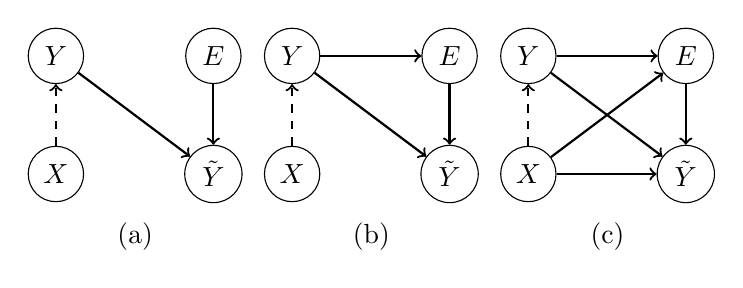
\begin{tikzpicture}[main_node/.style={circle,draw,minimum size=2em,inner sep=3pt]}]

     \node[main_node] (1) at (-1, 0) {$Y$};
     \node[main_node] (2) at (-1, -1.5)  {$X$};
     \node[main_node] (3) at (1, -1.5) {$\tilde{Y}$};
     \node[main_node] (4) at (1, 0) {$E$};
     \path[->,draw,thick]
     (1) edge node {} (3)
     (4) edge node {} (3)
     ;
    
     \path[->,dashed,thick]
     (2) edge node {} (1)
     ;
    
     \node[below=2cm] at (current bounding box.base) {(a)};
    
     \begin{scope}[xshift=3cm,grow=right,baseline]
     
     \node[main_node] (1) at (-1, 0) {$Y$};
     \node[main_node] (2) at (-1, -1.5)  {$X$};
     \node[main_node] (3) at (1, -1.5) {$\tilde{Y}$};
     \node[main_node] (4) at (1, 0) {$E$};

     \path[->,draw,thick]
     (1) edge node {} (3)
     (4) edge node {} (3)
     (1) edge node {} (4)
     ;
    
     \path[->,dashed,thick]
     (2) edge node {} (1)
     ;
    
     \node[below=2cm,xshift=1.5cm] at (current bounding box.base) {(b)};
    
     \end{scope}
    
     \begin{scope}[xshift=6cm,grow=right,baseline]
     \node[main_node] (1) at (-1, 0) {$Y$};
     \node[main_node] (2) at (-1, -1.5)  {$X$};
     \node[main_node] (3) at (1, -1.5) {$\tilde{Y}$};
     \node[main_node] (4) at (1, 0) {$E$};

     \path[->, draw,thick]
     (1) edge node {} (3)
     (4) edge node {} (3)
     (1) edge node {} (4)
     (2) edge node {} (3)
     (2) edge node {} (4)
     ;
    
     \path[->,dashed,thick]
     (2) edge node {} (1)
     ;
    
     \node[below=2cm,xshift=3cm] at (current bounding box.base) {(c)};
    
     \end{scope}
 \end{tikzpicture}
 }
 \end{figure}

\subsection{Loss factorization and correction}
    
Many label noise robustness methods can be found on literature, in this work we highlight the \textit{backward} and \textit{forward} loss corrections, proposed by \cite{Patrini2017} using concepts of loss factorization~\citep{Patrini2016}. Those loss correction techniques considers a NAR label noise, which is described by a transition matrix $T$ such as 
\begin{equation}
    T_{i,j} = P(\tilde{Y} = y_j|Y = y_i),
\end{equation}
where $\mathcal{Y} = \{y_1, y_2, \ldots, y_c\}$ is the set of all possible class labels. Transition matrix includes corruption probabilities for every possible label combination, each value represents the probability of one label be corrupted onto another. This matrix is row-stochastic and not necessarily symmetric across the classes.
\begin{equation} \label{eq:backward}
    \ell^{\leftarrow}(P(\tilde{Y}|X)) = T^{-1} \ell(P(\tilde{Y}|X))
\end{equation}

The backward loss correction is defined by Equation~\ref{eq:backward} to an arbitrary loss function $\ell$ and a transition matrix $T$. The backward loss correction involves a linear combination of the loss values for each observed label, using coefficients that depends on the probability that each observed label reflects the true class. Intuitively, we are reweighting the loss according to the noise probabilities of each label using the inverse of T and thus somehow going one step back, reverting the noise effects. This corrected loss is unbiased and can be minimized with any conventional back-propagation algorithm, making it flexible to include within different training techniques and data pipelines.
\begin{equation} \label{eq:forward}
    \ell^{\rightarrow}(P(\tilde{Y}|X)) = \ell(T^{\top} P(\tilde{Y}|X))
\end{equation}

However, backward correction requires matrix inversion, which may not exist or may lead to numerical instabilities if the transition matrix T is ill-conditioned. Although there is possible solutions to a bad condition number of T, one should consider using the forward correction, a backward variation proposed by \cite{Patrini2017} to avoid this issue, as defined in Equation~\ref{eq:forward}. While backward acts on the loss itself, forward corrects model predictions. Forward correction does not have the same theoretical guarantees as backward, but offers a label noise robustness, ensuring that the learned model is the minimize over the clean distribution without the need of matrix inversion.

\subsection{Fairness in the presence of noise}\label{sec:fairness_noise}

Some recent works deal with fairness problems in the presence of noise. For example, the sensitive attribute available could be noisy, which could distort the effects of fairness intervention. In this context, \cite{Lamy2019} uses noise-rate estimators from the label noise literature to change a fairness model. Also, \cite{Fogliato2020} proposes a framework for assessing how assumptions on the noise across groups affect the predictive bias properties in risk assessment models. Furthermore, \cite{Wang2020} considers the consequences of naively relying on noisy protected group labels while proposing two new optimization approaches with sensitive attribute noise robustness. A denoised version of the selection problem to deal with noisy sensitive attributes is proposed in \cite{Mehrotra2021}. Lastly, \cite{Celis2021} proposes an optimization framework for classification in the presence of noisy protected attributes.

There is also the perspective of dealing with the proxy features divergence or covariance. A theoretical approach to this issue identifying potential sources of errors can be found in \cite{Prost2021}. The problem of measuring group fairness in ranking based on divergence with proxy features is investigated by \cite{Ghazimatin2022}. A framework of fair semi-supervised learning in the pre-processing phase can be found in \cite{Zhang2022}, which includes predicting labels for unlabeled data, a resampling method, and ensemble learning to improve accuracy and decrease discrimination.

Another research direction is considering how fair models perform in the presence of NNAR label noise, where error rates of corruption depend both on the label class and the membership of a protected subgroup. In this scenario \cite{Wang2021} addresses the problem of fair classification and \cite{Wu2022} provides a general framework for rewriting the classification risk and the fairness metric in terms of noisy data and thereby building robust classifiers. In \cite{Ghosh2023} a study about the presence of noise in the protected attribute can be found.

Furthermore, many recent works deals with fairness under semi-supervised settings considering censored data, that is, for some individuals the class label is not available due censorship~\cite{WZhang2022,WZhang2023_a,WZhang2023_b,WZhang2023_c}. In this scenario, the main approach is to use some technique to estimate the missing data instead of removing the instance from training data. This is closely related to the previous problems of fair learning under noisy data. In censored fairness problems noise can be interpreted as a kind of censorship, as the original data affected by noise is not available.

Bias and noise are two related phenomena, both corrupt data affecting models trained with this data. For example, if noise disproportionately affects different groups this potentially produces unfairness in models that uses this data in training~\citep{Wang2021}. For example, we could have positive true class ($Y = 1$) flipped into negative labels ($\tilde{Y} =0$) more frequently in the protected group ($A = 1$) than in privileged group ($A = 0$). Simultaneously, the negative class ($Y = 0$) could be more frequently flipped into positives observed labels ($\tilde{Y} = 1$) within privileged/unprotected group ($A = 0$). This scenario could lead to a undetected higher false negative rate to protected group and higher false positive rate to privileged group. In this case the Noisy Not at Random data would be a source of negative social bias.

As refered before \cite{Mehrabi2019} a non-exhaustive list of bias types was presented. In the scenario described above, the incorrect measurement of the true class resulted in a different observed label ($Y \neq \tilde{Y}$), which could be classified as a \textit{Measurement Bias}. Similarly, a Noisy Not at Random data could lead to a \textit{Population Bias}, where the characteristics of the population represented in the data differ from those of the original target population.

It can be challenging to distinguish between label noise and bias in certain scenarios, specially when noise disproportionately affects different social groups. Although there is some overlapping, they are distinct phenomena. Label noise is a stochastic process that is considered independent and unintentional~\citep{Frenay2014}, whereas bias is rooted in historical and social issues and could be intentional. Furthermore, even noise-free data, correctly represented by observed features and labels, may be unfair since the social phenomena that produce this data could be biased against some groups. 

Prior studies in the realm of fairness have largely concentrated on understanding how noisy or censored data affects fair learning and on mitigating these effects. Thus, the objective of this work is not to theoretically deal with fair machine learning as a label noise problem or incorporate noisy classes or attributes in fairness problems. In contrast, our approach is inspired by label noise techniques, but with a distinct goal: not merely to analyze or mitigate the impact of noise or censorship, but to directly address and reduce unfairness itself.